%
% thesis
% @author Tobias Weber <tweber@ill.fr>
% @date jan-2021
% @license see 'LICENSE' file
%

\documentclass[english, 11pt]{book}

\RequirePackage{fixltx2e}
\RequirePackage{fix-cm}

\usepackage{amsmath}
\usepackage{tensor}
\usepackage{bm}
\usepackage{siunitx}
\usepackage{graphicx}
\usepackage[section]{placeins}
\usepackage{babel}
\usepackage[hyphens]{url}
\usepackage[numbib, chapter]{tocbibind}
\usepackage[colorlinks=true, linkcolor=black, citecolor=blue, urlcolor=blue, unicode=true]{hyperref}
\usepackage[a4paper]{geometry}
\geometry{tmargin=2.5cm, bmargin=2.5cm, lmargin=2cm, rmargin=2cm}

\renewcommand{\arraystretch}{1.25}

\makeatletter
% Bold math tip from Prof. Icking and https://tex.stackexchange.com/questions/209466/problem-with-tocloft-minitoc-and-bold-math-mode
\g@addto@macro\bfseries{\mathversion{bold}}
\makeatother


\begin{document}

\newcommand{\ill}{Institut Laue-Langevin (ILL), 71 avenue des Martyrs, CS 20156, 38042 Grenoble cedex 9, France}
\newcommand{\fuh}{Fernuniversit\"at in Hagen (FUH), Universit\"atsstraße 47, 58097 Hagen, Germany}


\title{Path-finding for triple-axis spectrometers}
\author{Tobias Weber, tweber@ill.fr}

\maketitle
\tableofcontents




% ====================================================================================================================================
%\part{Front matter}
%\addcontentsline{toc}{part}{Front matter} 
%
% project plan / abstract
% @author Tobias Weber <tweber@ill.fr>
% @date jan-2021
% @license see 'LICENSE' file
%

\chapter*{Abstract}
\addcontentsline{toc}{chapter}{Abstract}

The triple-axis spectrometer (TAS) \cite{Shirane2002} was invented by B. Brockhouse in the 1950s and 
is among the foremost measurement methods in the field of inelastic neutron scattering. 
It enables the probing of vibrational (phonon) or magnetic (magnon) excitations in single-crystals and allows 
mappings of their dispersion relations, i.e. their energy-momentum relation, $E\left( \underline{Q} \right)$.

The three axes of a TAS are offset by relative angles to one another, and comprise 
(i) the reactor-monochromator-sample axis, where a specific neutron energy is picked out of the polychromatic 
beam coming from the reactor's moderator; 
(ii) the monochromator-sample-analyser axis, whose angle selects a specific momentum transfer, $\underline{Q}$, 
from the neutron to the sample; and 
(iii) the sample-analyser-detector axis, which selects the energy transfer, $E$.

During the usual operation of a TAS, the user selects $\left( \underline{Q}, E \right)$ coordinates in the reciprocal (dual)
crystal space of the sample to be measured. While the vector space of crystal coordinates 
is in general non-Euclidean, crystal coordinates have a one-to-one correspondence with the axis angles 
of the TAS. The correspondence can be calculated by the so-called ``$UB$ matrix formalism'' \cite{Lumsden2005}. 
Here, $B$ is the transformation matrix from crystal to lab coordinates and $U$ is a rotation to a specific 
crystal plane. From that, the TAS angles can be derived using Bragg's law.

Due to angular constraints by cables and tubes, as well as spatial constraints from the crammed instrument space, 
not every $\left( \underline{Q}, E \right)$ coordinate point is accessible, and a careful mapping of each point is
usually required beforehand to avoid collisions of the instrument with walls, collisions with itself or movements
which could pull out fragile cables.

The goal of the proposed project is the development and implementation of a path-finding algorithm for 
neutron triple-axis spectrometers. Given a user-selected target coordinate in reciprocal crystal space, 
the algorithm will be able to navigate the instrument in its constrained angular space. The problem is similar to 
moving a robot arm around obstacles, with the addition of having the start and target coordinates in a 
coordinate system with a different metric.

%\begin{figure}[ht]
%	\begin{centering}
%	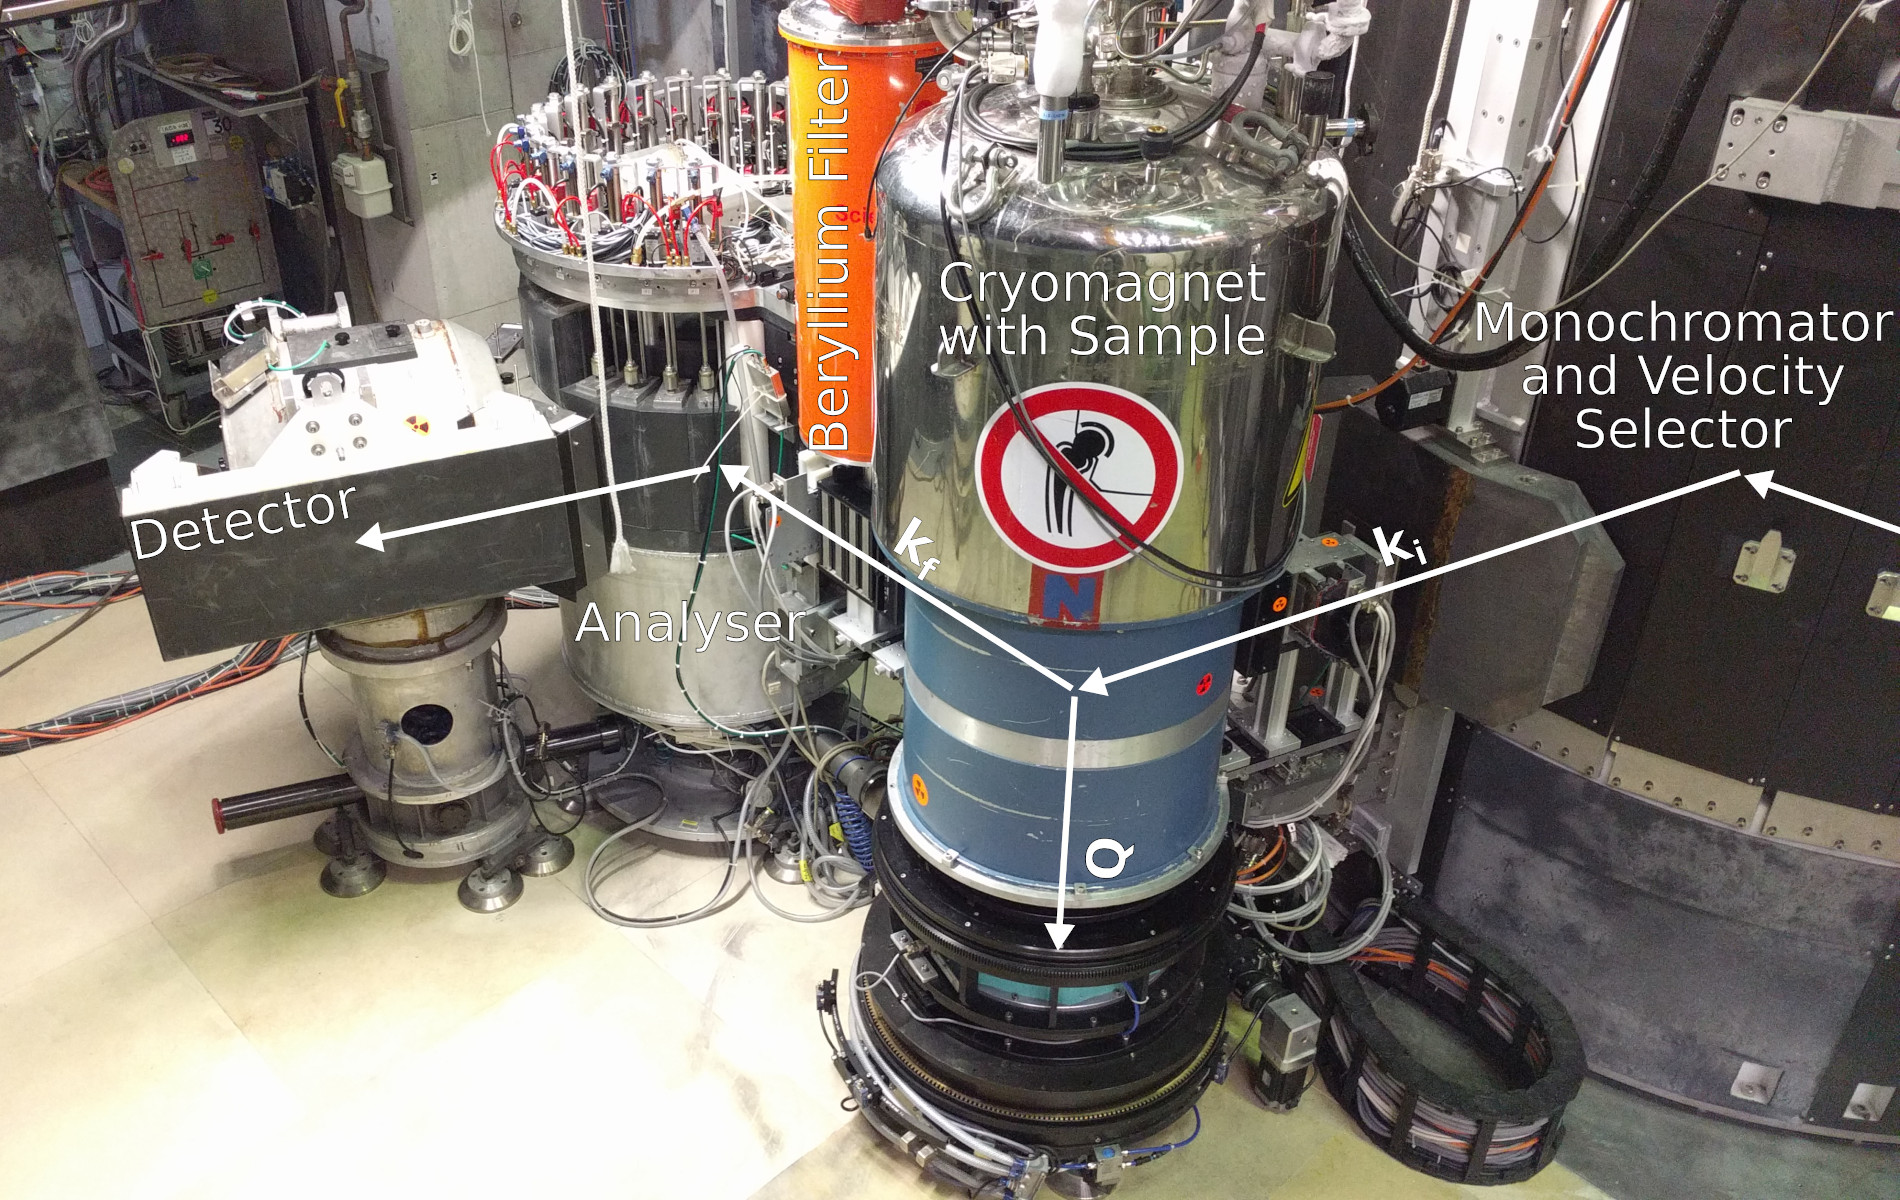
\includegraphics[width=0.66\textwidth]{figures/thales.jpg}
%	\end{centering}
%	\caption{The picture shows the triple-axis spectrometer \textit{ThALES} \cite{thales} at the ILL.}
%	\label{fig:tas}
%\end{figure}

%
% acknowledgements and thanks
% @author Tobias Weber <tweber@ill.fr>
% @date july-2021
% @license see 'LICENSE' file
%

\chapter*{Acknowledgements}
\addcontentsline{toc}{chapter}{Acknowledgements and Thanks}

I wish to thank my thesis advisors, Prof. Dr. Christian Icking and Dr. Lihong Ma, for accepting 
and supporting this project, for their advice and our regular discussions, the friendly atmosphere, 
as well as for always being available for questions.

Equal thanks to Dr. Martin B\"ohm, leader of the spectroscopy group at the ILL and instrument 
scientist at the Thales spectrometer, to Yannick Le Goc (computer scientist at the instrument 
control and electronics group), as well as Dr. Paul Steffens (Thales instrument scientist) for our 
regular discussions about various triple-axis automatisation projects, our experiments and the
instrumental aspects. I furthermore wish to thank Jérôme Locatelli (instrument control group) for
all the help with \textit{NOMAD}, the instrument control system at the ILL, and the technical discussions
about its internal details. 
Thanks to Dr. Paolo Mutti, the head of both the scientific computing and the instrument control group 
at the ILL, for supporting this project and for the great atmosphere and working environment there.

Also not to forget the continuing support from my former advisor for past theses, Prof. Dr. Peter B\"oni,
as well as from Prof. Dr. Christian Pfleiderer, Prof. Dr. Markus Garst, and Dr. Marc Janoschek in all our ongoing projects.

Financial support by the Institut Laue-Langevin via its \textit{P\^ole Formation} is gratefully acknowledged,
an I wish to thank Carole Fauchier for the administrative help.

Last but not least also many thanks to my family and to Soilhat for always being there for me!



%\part{Main part}

\chapter{Introduction}
%
% intro
% @author Tobias Weber <tweber@ill.fr>
% @date mar-2021
% @license see 'LICENSE' file
%

\chapter{Introduction}
\label{ch:intro}
In this first chapter, we introduce some basic concepts of neutron scattering and shortly present two types of
instruments typically found at research reactors (section \ref{sec:instruments}). A special emphasis is put
on triple-axis spectrometers (TAS) as the work-horse of inelastic neutron scattering. Finally, we summarise
the current state of autonomous experimentation (section \ref{sec:autonomous}).


\section{A brief history of neutron physics \label{sec:neutrons}}

The history of neutron physics begins in 1932 with the discovery of the neutron by James Chadwick, who used
alpha particles (helium nuclei) to bombard a beryllium-9 sample, thereby producing carbon-12 and one neutron
per reaction \cite[p. 1]{Jacrot2021}. The neutron that was created in this way was found to have a mass similar
to the proton ($m_n = 1.675\cdot10^{-27}\,\mathrm{kg}$, $m_p = 1.673\cdot10^{-27}\,\mathrm{kg}$), but, as the
name implies, no charge was detected \cite[p. 2]{Squires2012}. The absence of a charge makes the neutron very
useful for science, as it is subject to purely nuclear interactions with atomic nuclei, without any electrostatic
repulsion, for example by the electron hull \cite[p. 1]{Squires2012}.

In 1939, Otto Hahn used a Chadwick-type neutron source to irradiate uranium isotopes in an attempt to produce
heavy trans-uranium elements \cite{wiki_fission}. The measurements did not yield the expected results, because
instead of heavier elements, the experiment produced lighter elements. This was interpreted by Lise Meitner as
a splitting of the uranium nucleus, marking the discovery of nuclear fission \cite{wiki_fission}. A typical possible
channel of a fission reaction is the decay of uranium-235 into baryum-144 and krypton-89, where two to three
neutrons are produced by each reaction in addition to the daughter nuclei and energy \cite{wiki_fission}.

In 1942, Enrico Fermi made use of the excess neutrons that are obtained by each fission reaction to produce a
continuous, self-sustaining chain reaction in the first artificial nuclear reactor, the
\textit{Chicago Pile-1}~\cite[p.1]{Jacrot2021}.
It is interesting to note that while \textit{Chicago Pile-1} was the first \textit{artificial} nuclear reactor,
it was not the first one, strictly speaking. The first \textit{natural} reactor was discovered to have run more
than 1.5 billion years ago in Oklo, Gabun, at an average power of about 100 kW for a period of half a million
years \cite{wiki_oklo}.

The first research reactor, having a power of 3.5 MW~\footnote{As research reactors do not produce electricity,
the given numbers refer to thermal powers.} and being used for studies in solid-state physics, was built in
Oak Ridge, USA, in 1943, shortly after Fermi's pile \cite[p. 3]{Jacrot2021}.
Here, first neutron scattering experiments were performed by Clifford Shull using a two-axis diffractometer \cite[pp. 3, 37]{Jacrot2021}.

From there on, science advanced fast, and several centres dedicated to neutron research were founded around the world.
A selection of research reactors in operation today include the 20 MW \textit{Forschungsreaktor M\"unchen II}~\cite{web_mlz}
(FRM-II) at the Heinz-Maier-Leibnitz-Zentrum in Germany,
the 20 MW reactor at the NIST Center for Neutron Research~\cite{web_nist} (NCNR),
the 85 MW \textit{High Flux Isotope Reactor}~\cite{web_oakridge} (HFIR) at the Oak Ridge National Laboratory,
both based in the United States,
and the reactor of the Institut Laue-Langevin~\cite{web_ill} (ILL) in France, which - at 58 MW - is the most
powerful neutron source used for science in Europe.

Studying the structure and dynamics of crystals is made possible since neutrons emerging from the reactor can be
slowed down (moderated) into energy regions where their de Broglie wavelength $\lambda = h/p$ \cite[p. 89]{Gross2012}
corresponds to typical inter-atomic distances in crystal unit cells, which is of the order of 1 \AA{}ngstr\"om,
i.e. $10^{-10}$ m \cite[pp.1,3]{Squires2012}. In the formula, $p$ denotes the neutron momentum and $h$ Planck's constant.
Such a slowing-down of neutrons is usually performed using a secondary moderator outside the reactor's main moderator --
which itself sustains the nuclear fission -- for example using liquid $\mathrm{D_2O}$ \cite[p. 82]{Jacrot2021}.
Here, neutrons are brought into a new thermal equilibrium by elastic collisions with the nuclei of the moderator's
atoms \cite[p. 30]{Stacey2007}, i.e. the neutrons take the temperature and thus energy of the surrounding material.



\section{Instruments for neutron scattering \label{sec:instruments}}

While a modern research reactor houses a multitude of different instrument types, among them time-of-flight,
back-scattering and spin-echo spectrometers, furthermore Larmor, Laue and small-angle diffractometers, in
this section, we instead want to shortly present the most basic types of instrument, the two-axis diffractometer
and the triple-axis spectrometer. Together, the discovery of these two instruments by Clifford Shull and Bertram Brockhouse,
respectively, was awarded the 1994 Nobel Prize in Physics~\cite{web_nobel1994}.
A comprehensive introduction into these instruments, especially triple-axis spectroscopy, can be found in the
book by G. Shirane \cite{Shirane2002}. An advanced treatment of neutron scattering theory is given by
G. L. Squires \cite{Squires2012}.


\subsection{Two-axis diffractometers}

A two-axis diffractometer is used for determining the static structure of crystals, which are here typically provided
in powder form, but can also be single-crystals. It is the single most fundamental kind of machines in the field of
neutron scattering at research reactors. This instrument type consists of a single-crystal (meaning it comprises one
single grain), which is called ``monochromator'' and named after its function to pick out one specific wavelength,
$\lambda_i$, from the polychromatic neutron beam coming from the reactor core or from one of its moderators.
The physical principle behind wavelength selection is Bragg reflection \cite[p. 68]{Gross2012} \cite[p. 13]{Shirane2002},
\begin{equation}
	\label{eq:bragg}
	n \cdot \lambda_i \ =\  2 d \cdot \sin\left( \theta_M \right),
\end{equation}
with $\lambda_i$ being the neutron wavelength, $d$ the spacing of the crystal lattice planes from which scattering
takes place, $\theta_M$ half the monochromator scattering angle and $n$ the order of the reflection. A graphical
interpretation of Eq. \ref{eq:bragg} is depicted in Fig. \ref{fig:braggscattering}.

\begin{figure}[htb]
	\centering
	\includegraphics[width=0.35\textwidth]{figures/bragg.pdf}
	\caption[Bragg scattering.]{
		Bragg scattering on crystal planes having a spacing $d$. An incoming parallel neutron beam is reflected at an
		angle $2 \cdot \theta_M$ on both the upper and lower crystal plane, leading to a path difference of
		$2d \sin\theta$ between the beams. If the path difference is an integer multiple of the neutron wavelength,
		$\lambda_i$, the beams interfere constructively. Figure drawn after \cite[p. 68, Fig. 2.7]{Gross2012}. }
	\label{fig:braggscattering}
\end{figure}

The resulting monochromatic beam with the wavelength $\lambda_i$ and wavevector $\underline{k}_i$ is Bragg-scattered
a second time, this time from a sample powder containing small crystallites. Diffractometers typically contain hundreds
of neutron detectors surrounding the sample and picking up diffracted neutrons at a whole range of scattering angles
$2 \theta_S$. The scattering angles define the momentum transfer from the neutron to the sample as \cite[p. 11]{Shirane2002}
\begin{equation}
	\label{eq:Q}
	\hbar \underline{Q} \ =\  \hbar \left( \underline{k}_i - \underline{k}_f \right),
\end{equation}
where the two wavevectors $\underline{k}_i$ and $\underline{k}_f$ point along the propagation directions of the neutrons
before and after scattering from the sample, respectively. They both have the same magnitudes for diffraction, namely
$k_{i,f} = 2\pi / \lambda_i$ and are rotated by $2\theta_S$ from one another, see Fig. \ref{fig:diffraction} for a visualisation.
The symbol $\hbar$ denotes the reduced Planck's constant, $\hbar = h / \left( 2\pi \right)$.

\begin{figure}[htb]
	\centering
	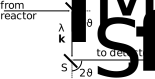
\includegraphics[width=0.35\textwidth]{figures/diffraction.pdf}
	\caption[Neutron diffraction.]{
		Principle of neutron diffraction. A polychromatic neutron beam coming from the reactor core is Bragg-scattered
		from the monochromator (M), picking out a single wavelength $\lambda_i$ and corresponding wavevector $\underline{k}_i$.
		The monochromatic beam is next scattered on the sample (S) at an angle $2\theta_S$, defining the direction of a
		wavevector $\underline{k}_f$. The momentum transferred from the neutron to the sample is given by Eq. \ref{eq:Q}
		as the difference of the two wavevectors.}
	\label{fig:diffraction}
\end{figure}

By the intensity of the sample's Bragg reflections, each of which appears at a different scattering angle $2\theta_S$
and thus momentum transfer $\hbar \underline{Q}$, the so-called static nuclear structure factor \cite[p. 25]{Shirane2002}
can be reconstructed. Absences of Bragg peaks determine the crystal symmetry given by its space group. Together,
they determine the structural build-up of the crystal.


\subsection{Triple-axis spectrometers}

In a two-axis diffractometer the scattering angle from a sample defines a momentum $\hbar \underline{Q}$ which is
transferred from the the neutron to the sample. It does not allow to select a sample-neutron energy transfer,
which is given by the de Broglie equation as \cite[p. 89]{Gross2012} \cite[p. 11]{Shirane2002}
\begin{equation}
	\label{eq:E}
	E \ =\ E_i - E_f \ =\ \frac{\left( \hbar k_i \right)^2}{2 m_n} - \frac{\left( \hbar k_f \right)^2}{2 m_n}.
\end{equation}
The constant $m_n$ is the neutron mass, for elastic scattering $k_i = k_f$.
The data obtained from such an instrument is instead integrated over all possible energy transfers.
This is no problem in practice, because elastic scattering, i.e. scattering with no energy transfer,
is usually many orders of magnitude stronger than inelastic scattering and any inelastic contribution
would not hide the elastic signals used for crystal structure determination.

Complementary to the two-axis instrument, a triple-axis spectrometer (TAS) is usually not used to study structures,
but instead measures the dynamics of the sample crystal. The samples used at TAS are usually in single-crystalline form.
At TAS machines, we are only interested in non-zero energy transfers, i.e. the cases when neutrons scattering from the
sample crystal excite collective modes. These modes typically comprise vibrations of the crystal's nuclei, called phonons,
which can be imagined as quantised sound waves \cite[pp. 123-137]{Shirane2002}. Another typical example includes the
coupled motions of the atom hull's electron spins, which are named spin-waves or magnons \cite[pp. 137-144]{Shirane2002}.

As the name implies, the difference of the TAS set-up compared to the two-axis diffractometer is one additional axis.
Having passed the sample, the neutrons may have changed their energy and thus wavelength and magnitude of the wavevector.
A further single-crystal is placed in the neutron path between the sample and the detector. Bragg scattering on this crystal
allows the detection of the neutron wavelength $\lambda_f$ after the sample, which remained unknown in the diffractometer.
Since we also know the incoming wavelength $\lambda_i$ before the scattering event at the sample, we can calculate the
transferred energy as given by Eq. \ref{eq:E}. This additional crystal and the corresponding instrument axis are named ``analyser''.
Fig. \ref{fig:spectroscopy} visualises the principles of the instrument, Fig. \ref{fig:thales} shows a typical triple-axis
instrument with its three axes, namely the monochromator in the right-hand side of the picture, the sample and the analyser
with the attached detector.

\begin{figure}[htb]
	\centering
	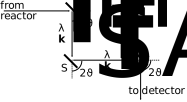
\includegraphics[width=0.4\textwidth]{figures/spectroscopy.pdf}
	\caption[Neutron spectroscopy.]{
		Principle of neutron spectroscopy. A polychromatic neutron beam coming from the reactor core is Bragg-scattered
		from the monochromator crystal (M), picking out a single wavelength $\lambda_i$ and wavevector $\underline{k}_i$.
		The monochromatic beam is next scattered on the sample (S) at an angle $2\theta_S$, defining a wavevector $\underline{k}_f$.
		The magnitude of $\underline{k}_f$ and thus $\lambda_f$ is determined by Bragg-scattering on the analyser crystal (A).
		The momentum and energy transfers are given by Eqs. \ref{eq:Q} and \ref{eq:E}, respectively. }
	\label{fig:spectroscopy}
\end{figure}

\begin{figure}[htb]
	\centering
	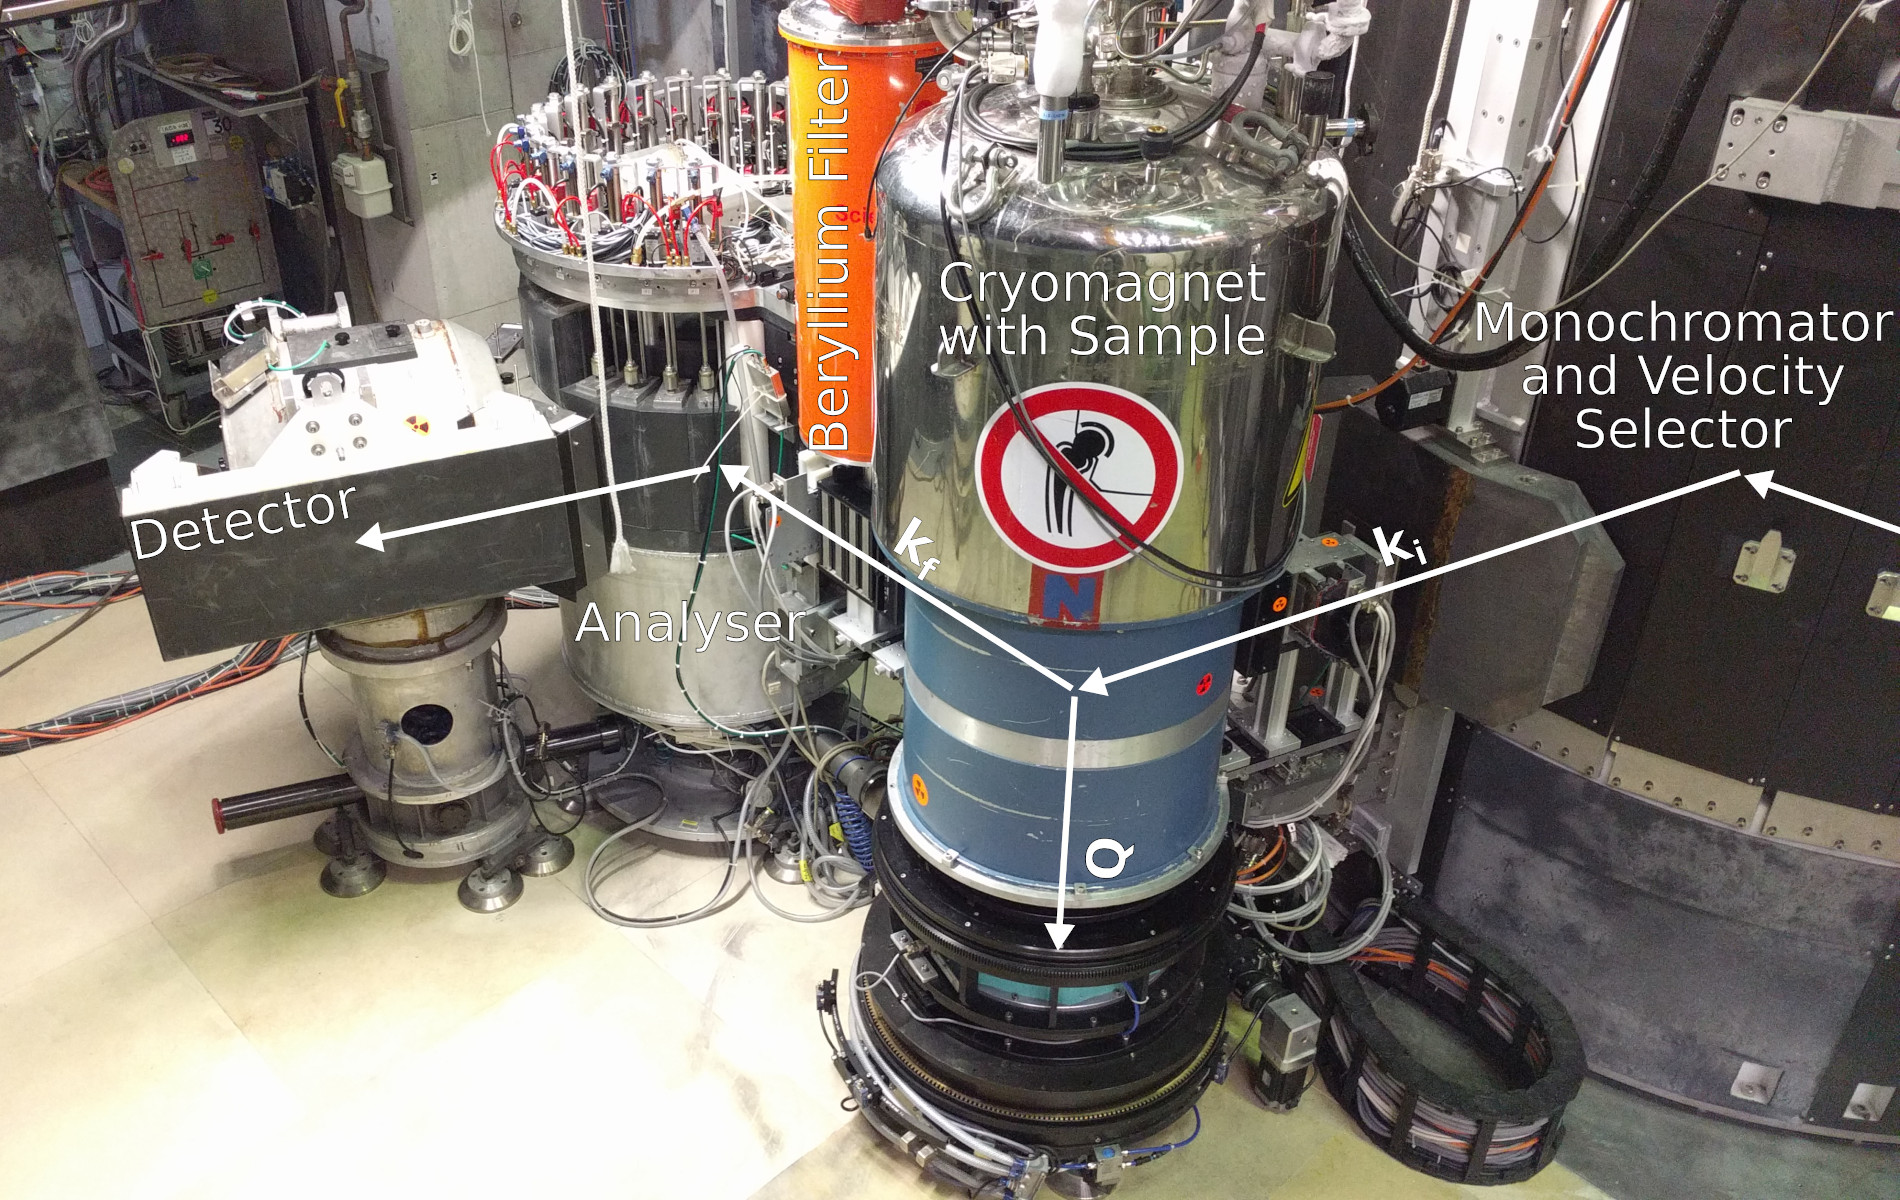
\includegraphics[width=0.75\textwidth]{figures/thales.jpg}
	\caption[The Thales instrument at the ILL.]{
		The triple-axis spectrometer ThALES \cite{thales} at the Institut Laue-Langevin in Grenoble, France. The neutron
		path from the reactor to the detector is marked as white arrows. The momentum transfer, $\hbar \underline{Q}$,
		is also shown. This picture is reproduced from the supplementary information of Ref. \cite{skxpaper}.}
	\label{fig:thales}
\end{figure}



\section{Autonomous experiments \label{sec:autonomous}}

Up until the end of 2019, TAS experiments usually required external scientists to stay at the research reactor for
typically one week and conduct the experiment together with the instrument's responsible scientists. Specifically
at the Institut Laue-Langevin (ILL), there had already been attempts \cite{Song2020} of the instrument control
and scientific computing groups to convince the instrument scientists of the benefits of instrumentation with full- or
semi-autonomous as well as remote control. Nevertheless, the impact had been limited.
Virtual experiments, on the other hand, had already been established in the simulation of actual experiments and in their
planning phase. Noteworthy software systems are \textit{McStas} \cite{McStas2020, McStas2021}, a neutron ray-tracing software based on the
Monte-Carlo method, simulating a large number of random neutrons and their interaction with various neutron-optical components,
as well as the software \textit{vTAS} \cite{vTAS2013}, which simulates the angles and crystal coordinates of a triple-axis
instrument and also provides support for calculating collisions with walls.

The situation changed significantly with the Covid-19 pandemic. Receiving visiting scientists from other countries had
not been possible anymore, or only to a very limited degree. Instead, remote experimentation and instrument control has
now become the new norm, with users connecting to a web interface from which the experiment can be planned and data can
be analysed~\cite{web_ill_visa}.
Discussions with instrument scientists take place via web-cams that have been installed at every instrument.

At the same time, the idea to automate manual tasks at instruments using algorithms and artificial intelligence has
gained significant traction, with first autonomous experiments being attempted at the ILL's spectroscopy group
\cite{web_ill_autonomous2020, Noack2021}.

As part of the current drive towards autonomous experimentation at the ILL, the goal of the present work is the design
and implementation of a software tool which enable an automatic path-finding for TAS instruments. Path-finding
is necessary for the instrument to circumvent obstacles in its way and for safe, collision-free movement close to walls.
Currently, this task has to be performed by the instrument scientists before each new scan series in a time-consuming fashion.
The current approach requires the instrument to be driven along the programmed scan path, but without measuring and with
the neutron beam from the reactor closed.
The scientist has to stay in the instrument space and watch the instrument as it moves to every scan position.
A manual stop has to be initiated when the instrument would collide with a wall, with itself, or when the rotation of one
of the axes would pull out a cable or tube.

An early attempt at automatic collision prevention and path-finding for a triple-axis spectrometer can be found in 
the 2006 work by M\"uhlbauer and Hradil \cite{Muehlbauer2006}, but their method is based on a simple grid search and thus
does not result in paths which keep the furthest distance to obstacles. A reason for such a solution might be
that computing power was not sufficient at that time to calculate the mesh of possible paths as it is 
done with the algorithms to be presented in the current work.



\section{Summary}

This chapter provided a short glance at neutron physics and the types of instrument typically used at research
reactors, with special emphasis on the triple-axis spectrometer. The complexity of the movement of these kind of
instruments necessitate the use of a path-finding system for a more effective set-up of measurements.
In the next chapter, we will introduce the coordinate systems used in crystallography and at TAS instruments,
and show how one set of coordinates transforms into the other.


\chapter{Crystal and Instrument Coordinate Systems}
\label{ch:xtal}
%
% xtal formulas
% @author Tobias Weber <tweber@ill.fr>
% @date 13-jul-2018
% @license see 'LICENSE' file
%

\chapter{Crystal and Instrument Coordinate Systems}
\label{ch:xtal}

In this chapter we review the theory for conversion between crystal coordinates and scattering angles 
at the triple-axis instrument. Section \ref{sec:xtalcoords} introduces crystal coordinates and the so-called 
$UB$ matrix formalism, section \ref{sec:tasangles} calculates the corresponding TAS angles. 
The formalisms \cite{Lumsden2005} reviewed here are ubiquitous in neutron science, they are not only used 
in the control programs of triple-axis instruments, among them \textit{NOMAD} \cite{web_NOMAD} 
or \textit{NICOS} \cite{web_NICOS}, but are also employed in virtual instrument simulators like \textit{vTAS} \cite{vTAS2013} or 
\textit{McStas} \cite{McStas2020}, as well as in data analysis software like \textit{Mantid} \cite{Arnold2014}.

Note that this chapter has already been published in the manual of the software from Ref. \cite{Takin2021},
as well as in my (physics) PhD thesis \cite[pp. 139-143]{PhDWeber},
where the latter featured an earlier version of the same text, figures, and derivations.
Originally, these formulas were re-derived with the aid of the source
code of \textit{McStas'} \textit{templateTAS} virtual instrument \cite{web_mcstas_templateTAS, McStas2020}.


% ------------------------------------------------------------------------------------------------------------------------------------
\section{Fractional crystal coordinates \label{sec:xtalcoords}}

We begin by presenting the so-called $UB$ matrix formalism to convert between relative lattice units 
of a crystal and laboratory coordinates used in instrument space. This method has been described in 
Ref. \cite{Lumsden2005}. The derivation of the transformation matrices, $A$ and $B$, describing fractional
crystal coordinates, can be found in \cite{wiki_fractional}, which we follow here.

\subsection{$A$ and $B$ matrices}
\paragraph{Real-space crystal lattice}
The unit cell of the crystal is spanned by its three basis vectors $\left| a \right>$, $\left| b \right>$, and $\left| c \right>$, 
which -- in general -- are not perpendicular to one another, but instead enclose angles of $\alpha$, $\beta$, 
and $\gamma$, respectively, as shown in Fig. \ref{fig:cell}. 
To calculate the crystallographic $A$ matrix which transforms non-orthogonal crystal to orthogonal lab units, 
we first need to reduce the number of parameters.
The respective relations between the three basis vectors and their angles can be directly obtained via
their scalar products, where we follow the derivation in Ref. \cite{wiki_fractional}:

\vspace{\abovedisplayskip}
\begin{minipage}{0.317\textwidth}
	\begin{equation} \left< a | b \right > \ =\  ab \cos \gamma, \label{eq:ab} \end{equation}
\end{minipage}
\begin{minipage}{0.317\textwidth}
	\begin{equation} \left< a | c \right > \ =\  ac \cos \beta, \label{eq:ac} \end{equation}
\end{minipage}
\begin{minipage}{0.317\textwidth}
	\begin{equation} \left< b | c \right > \ =\  bc \cos \alpha. \label{eq:bc} \end{equation}
\end{minipage}
\vspace{\belowdisplayskip}

\begin{figure}
	\centering
	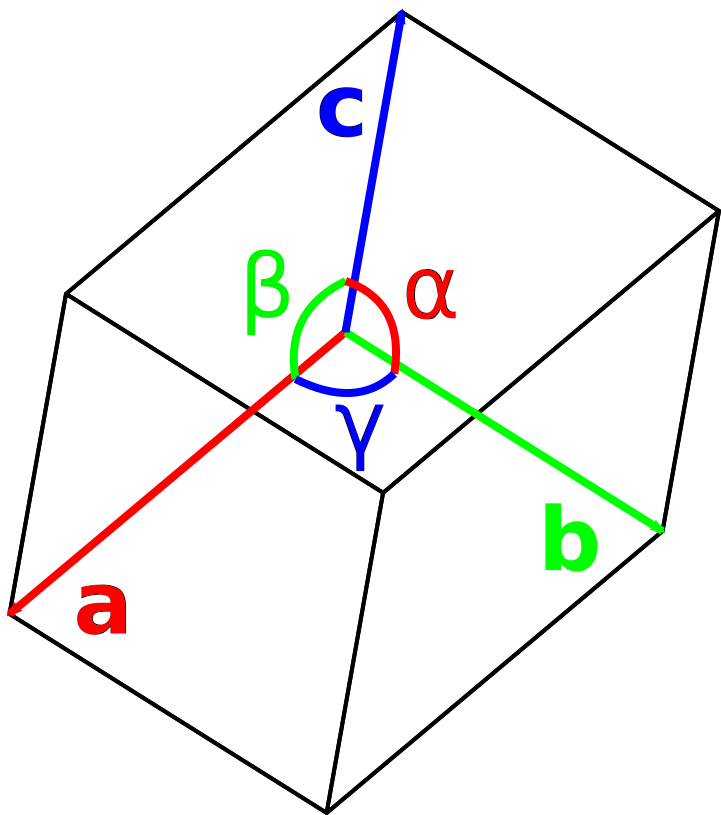
\includegraphics[width = 0.2 \textwidth]{figures/cell}
	\caption[Crystal unit cell.]{
		The unit cell of a crystal is given by its coordinate vectors $a$, $b$, and $c$ 
		as well as their angles $\alpha$, $\beta$, and $\gamma$.
		Figure drawn after the figure in Ref. \cite{wiki_fractional}.}
	\label{fig:cell}
\end{figure}


%\subsection*{Basis vectors}

The next goal is to explicitly write the components of the vectors $\left| a \right>$, $\left| b \right>$, and $\left| c \right>$ 
in terms of their lengths $a = \sqrt{\left< a | a \right>}$, $b = \sqrt{\left< b | b \right>}$, $c = \sqrt{\left< c | c \right>}$,
and the three angles.
To that end, we first choose -- without loss of generality -- $\left| a \right>$ along the $x$ axis, $\left| b \right>$ in the 
$xy$ plane, and $\left| c \right>$ in general:
\begin{equation} 
	\boxed{ \left| a \right> \ =\  \left( \begin{array}{c} a_1 = a \\ 0 \\ 0 \end{array} \right), }
	\hspace{0.5cm} \left| b \right> \ =\  \left( \begin{array}{c} b_1 \\ b_2 \\ 0 \end{array} \right),
	\hspace{0.5cm} \left| c \right> \ =\  \left( \begin{array}{c} c_1 \\ c_2 \\ c_3 \end{array} \right).
\end{equation}


Inserting $\left| a \right>$ and $\left| b \right>$ into Eq. \ref{eq:ab} gives the first component
of the $\left| b \right>$ vector:
\begin{equation} \left< a | b \right > \ =\  a_1 b_1 \ =\  ab \cos \gamma
\hspace{0.5cm} \Rightarrow \hspace{0.5cm} b_1 \ =\  b \cos \gamma. \end{equation}


Using the cross product between $\left| a \right>$ and $\left| b \right>$, we get the second component of $\left| b \right>$:
\begin{equation} 
	\left\Vert \left| a \right> \times \left| b \right> \right\Vert \ =\ 
	\left\Vert \left( \begin{array}{c} 0 \\ 0 \\ a_1 b_2 \end{array} \right) \right\Vert \ =\ 
	ab \sin \gamma \label{eq:crossab}
	\hspace{0.5cm} \Rightarrow \hspace{0.5cm} b_2 \ =\  b \sin \gamma.
\end{equation}

The vector $\left| b \right>$ is now complete:
\begin{equation} 
\boxed{ \left| b \right> \ =\  \left( \begin{array}{c} b \cos \gamma \\ b \sin \gamma \\ 0 \end{array} \right). } 
\label{eq:bvec} 
\end{equation}


Inserting $\left| a \right>$ and $\left| c \right>$ into Eq. \ref{eq:ac} gives the first component of $\left| c \right>$:
\begin{equation} \left< a | c \right > \ =\  a_1 c_1 \ =\  ac \cos \beta
\hspace{0.5cm} \Rightarrow \hspace{0.5cm} c_1 \ =\  c \cos \beta.
\end{equation}



Inserting $\left| b \right>$ and $\left| c \right>$ into Eq. \ref{eq:bc} yields the second component of $\left| c \right>$:
\begin{equation} \left< b | c \right > \ =\  b_1 c_1 + b_2 c_2 \ =\  bc \cos \alpha, \end{equation}
\begin{equation} b \cos \gamma \cdot c \cos \beta + b \sin \gamma \cdot c_2 \ =\  bc \cos \alpha
	\hspace{0.5cm} \Rightarrow \hspace{0.5cm}
	c_2 \ =\  \frac{c \cos \alpha - c \cos \gamma \cos \beta}{\sin \gamma}. \end{equation}



The last component, $c_3$, can be obtained from the vector length normalisation, $ \left< c | c \right> = c^2 $:
\begin{equation} \left< c | c \right > \ =\  c_1^2 + c_2^2 + c_3^2 \ =\  c^2, \end{equation}
\begin{equation} c_3^2 \ =\  c^2 - c_1^2 - c_2^2
	\hspace{0.5cm} \Rightarrow \hspace{0.5cm}
	c_3^2 \ =\  c^2 \left[1 - \cos^2 \beta - \left(\frac{\cos \alpha - \cos \gamma \cos \beta}{\sin \gamma} \right)^2 \right].
\end{equation}

The full vector $\left| c \right>$ is now reads:
\begin{equation} \boxed{ \left| c \right> \ =\  \left( \begin{array}{c}
	c \cdot \cos \beta \\
	c \cdot \frac{\cos \alpha - \cos \gamma \cos \beta}{\sin \gamma} \\
	c \cdot \sqrt{ \sin^2 \beta - \left(\frac{\cos \alpha - \cos \gamma \cos \beta}{\sin \gamma} \right)^2 }
\end{array} \right). } \end{equation}



The crystallographic $A$ matrix, which transforms real-space fractional to lab coordinates (\AA) \cite{Lumsden2005},
is formed with the basis vectors in its columns \cite[p. 631]{Arens2015}:
\begin{equation}
	A \ =\  \left(
		\begin{array}{ccc}
			\left| a \right> & \left| b \right> & \left| c \right>
		\end{array}
	\right).
\end{equation}
Explicitly written out using the basis vectors, the matrix reads \cite{wiki_fractional}:
\begin{equation}
	A \ =\  \left(
		\begin{array}{ccc}
			\begin{array}{c} a \\ 0 \\ 0 \end{array}
			& 
			\begin{array}{c} b \cos \gamma \\ b \sin \gamma \\ 0 \end{array} 
			& 
			\begin{array}{c}
				c \cdot \cos \beta \\
				c \cdot \frac{\cos \alpha - \cos \gamma \cos \beta}{\sin \gamma} \\
				c \cdot \sqrt{ \sin^2 \beta - \left(\frac{\cos \alpha - \cos \gamma \cos \beta}{\sin \gamma} \right)^2 }
			\end{array}
		\end{array}
	\right).
\end{equation}


\paragraph{Reciprocal-space crystal lattice}
For calculations in solid-state physics and neutron scattering, one does not normally use
the real-space crystal lattice, but instead thinks in term of the so-called reciprocal-space
lattice \cite[pp. 11-15]{Shirane2002}.
Reciprocal space is constructed in a way to facilitate calculations with momenta on a periodic lattice,
for that reason it is also sometimes called momentum or Fourier space.
A comparison of the same Bragg scattering in real vs. reciprocal space is shown in Fig. \ref{fig:braggscattering_recip}.
It is obvious that the reciprocal view greatly simplifies the image: Bragg scattering on what is a set of parallel
crystal planes in real space in panel (a) becomes a single point in reciprocal space \cite[p. 66]{Gross2012},
the so-called Bragg peak $\left| G \right>$ in panel (c). The reciprocal vector $\left| G \right>$ is
perpendicular to the original crystal planes and its length is related to their distance $d$ by
$\left\Vert G \right\Vert = 2\pi/d$ \cite[p. 66]{Gross2012}. Panel (c) also shows how the lattice vector
together with the neutron beam directions forms the so-called scattering triangle, which is 
ubiquitous in visualisations of neutron scattering geometry \cite[pp. 14-15]{Shirane2002} and which will be 
discussed in the next section.
\begin{figure}[htb]
	\centering
	\includegraphics[width=1\textwidth]{figures/bragg_recip}
	\caption[Real and reciprocal lattice scattering.]{
		(a) Bragg scattering on crystal planes having a spacing $d$, viewed from real space.
			Figure drawn after Ref. \cite[p. 68, Fig. 2.7]{Gross2012}.
		(b) A view mixing real and reciprocal space. The reciprocal lattice vector, $\underline{G}$,
			is perpendicular to the real space crystal planes.
		(c) Bragg scattering viewed from reciprocal space. The direction of the incoming and outgoing
			neutron beams define wavevectors $\underline{k}_i$ and $\underline{k}_f$.
			Such a representation is called a scattering diagram or scattering triangle
			\cite[p. 14, Fig. 1.5]{Shirane2002}.}
	\label{fig:braggscattering_recip}
\end{figure}

From the construction of reciprocal space, it can be shown that the basis vectors of reciprocal space
are mutually perpendicular to the corresponding real space basis vectors \cite[p. 60]{Gross2012}.
This directly leads to the so-called $B$ matrix, which transforms reciprocal-space relative lattice units (rlu)
to lab coordinates (1/\AA) \cite{Lumsden2005}, is \cite[p. 60]{Gross2012}:
\begin{equation} B \ =\  2 \pi A^{-t}, \end{equation}
where $-t$ denotes the transposed inverse.
We can now also determine the metric tensor \cite[pp. 807-809]{Arens2015} corresponding to the coordinate
system defined by the $B$ transformation matrix, it reads \cite[p. 808]{Arens2015}:
\begin{equation}
	\left(g_{ij}\right) \ =\  \left<\underline{b}_i | \underline{b}_j \right> \ =\  B^T B,
\end{equation}
where the reciprocal basis vectors $\left| \underline{b}_i \right>$ form the columns of $B$ \cite[p. 631]{Arens2015}.

A rigorous introduction into the reciprocal crystal lattice can be found in the book by Gross
and Marx \cite[pp. 58 - 67]{Gross2012}.


\subsection{Example: lengths and angles in the reciprocal lattice}
Having a metric makes it straightforward to calculate lengths and angles.
The length of a reciprocal lattice vector $\left| G \right>$ seen from the lab system is 
(in 1/\AA{} units) \cite[p. 808]{Arens2015}:
\begin{equation}
	G  \ =\ 
	\left\Vert \left< G | G \right> \right\Vert \ =\  \sqrt{\left< G | G \right>}
		\ =\  \sqrt{G_i G^i} \ =\  \sqrt{g_{ij} G^i G^j}.
\end{equation}
The angle $\theta$ between two Bragg peaks $\left| G \right>$ and $\left| H \right>$ 
is given by their dot product \cite[p. 808]{Arens2015}:
\begin{equation}
	\frac{\left< G | H \right>}{\left\Vert \left< G | G \right> \right\Vert
		\cdot \left\Vert \left< H | H \right> \right\Vert} \ =\
	\frac{g_{ij} G^i H^j }{\sqrt{g_{ij} G^i G^j} \sqrt{g_{ij} H^i H^j}} \ =\  \cos \theta.
\end{equation}

Please note that if an index appears twice, both as subscript as well as a superscript, 
a summation over it is implied, see Ref. \cite{wiki_summation}.


\subsection{$U$ matrix}
The $B$ matrix alone yields the transformation from the non-orthogonal and reciprocal crystal 
coordinate system into the orthogonal lab units \cite{Lumsden2005}.
However, it does not yet take into account the actual rotation of the crystal so that a specific plane, 
the so-called scattering plane, can be accessed by the two-dimensional movements of the instrument. 
Such a rotation is performed by the $U$ matrix, whose rows contain two vectors inside the desired 
scattering plane and the plane normal \cite{Lumsden2005}.
These basis vectors are usually chosen along two orientation Bragg reflections \cite[pp. 87-88]{Shirane2002}
and are expressed in the orthogonal lab system, i.e. they are pre-multiplied by $B$.
For $U$ to be a rotation matrix, the basis vectors are normalised using, for instance, the
Gram-Schmidt algorithm \cite[p. 744]{Arens2015} \cite[pp. 269-270]{Arfken2013} or 
QR decomposition \cite[pp. 269-272]{Scarpino2011}.

In summary, a coordinate point $\left|Q_{\mathrm{rlu}}\right>$, which is given in relative lattice 
units of the reciprocal crystal, 
is transformed by the $B$ matrix into the orthogonal lab units used at the instrument \cite{Lumsden2005}.
It is then rotated by the $U$ matrix to account for the actual crystal orientation \cite{Lumsden2005}:
\begin{equation}
	\left|Q_{\mathrm{lab}}\right> \ =\  U \cdot B \cdot \left|Q_{\mathrm{rlu}}\right>.
	\label{eq:UBtrafo}
\end{equation}
In the rest of this work we will not use the $U$ matrix explicitly, though, but instead directly work 
with its basis vectors and the metric tensor. This is just a formality, though, the mathematics are the same.

% ------------------------------------------------------------------------------------------------------------------------------------




% ------------------------------------------------------------------------------------------------------------------------------------
\section{Scattering triangle and TAS angles \label{sec:tasangles}}

With the metric tensor \cite[pp. 807-809]{Arens2015} of the crystal coordinate system, we can now calculate the scattering angles
$2 \theta_M$, $2 \theta_S$, and $2 \theta_A$ from the monochromator, sample and analyser, respectively. 
The derivation of basic scattering geometries in triple-axis spectrometers can be found in \cite[Ch. 1.3]{Shirane2002},
which we follow here. 
The explicit calculation of the TAS angles based on the $UB$ formalism was originally presented in Ref. \cite{Lumsden2005}.

For the monochromator and analyser, the crystal angles $\theta_M$ and $\theta_A$ are coupled to 
their scattering angles, they are simply half their value, because the Bragg condition of Eq. \ref{eq:bragg}
always has to be fulfilled.
The crystal rotation for the sample is not necessarily half its scattering angle, $\Theta_S \ne 2\theta_S/2$, 
though, because the instrument can be freely positioned at any point of reciprocal crystal space.

The monochromator and analyser scattering angles follow directly from Bragg's equation 
\cite[p. 68]{Gross2012} \cite[p. 13]{Shirane2002}:

\begin{minipage}{0.45\textwidth}
	\centering
	\begin{equation} 2 d_{M}\sin \theta_{M} \ =\  n \lambda_{i}, \end{equation}
	\begin{equation} 2 k_{i} \sin \theta_{M} \ =\  2 \pi n / d_{M}, \end{equation}
	\begin{equation} \boxed{ \theta_{M} \ =\  \arcsin \left( \frac{\pi n}{d_{M} \cdot k_{i}} \right). } \end{equation}
\end{minipage}
\begin{minipage}{0.45\textwidth}
	\centering
	\begin{equation} 2 d_{A}\sin \theta_{A} \ =\  n \lambda_{f}, \end{equation}
	\begin{equation} 2 k_{f} \sin \theta_{A} \ =\  2 \pi n / d_{A}, \end{equation}
	\begin{equation} \boxed{ \theta_{A} \ =\  \arcsin \left( \frac{\pi n}{d_{A} \cdot k_{f}} \right). } \end{equation}
\end{minipage}

%\vspace{0.5cm}

To determine the sample scattering angle $2 \theta_S$, we use the so-called scattering triangle, see 
Fig. \ref{fig:scattering_triangle}, whose connection to the neutron beam direction has already 
been established in the previous section.
The scattering triangle can be directly determined by the angles the instrument is positioned at \cite[pp. 14-15]{Shirane2002}: 
For that, we have a look at the incoming and final neutron wavevectors $\left| k_i \right>$ and $\left| k_f \right>$, 
whose directions (but not lengths!) correspond directly to the neutron paths before and after the sample, 
respectively, as shown on the left-hand side of Fig. \ref{fig:scattering_triangle}. We can rearrange them so 
that their tips meet, as depicted on the right-hand side of Fig. \ref{fig:scattering_triangle}, where the 
scattering triangle is formed by $\left| k_i \right>$ and $\left| k_f \right>$ together with the
scattering vector $\left| Q \right> = \left| k_i \right> - \left| k_f \right>$ \cite[p. 14]{Shirane2002}.
Here, the two wavevectors enclose the scattering angle $2 \theta_S$.

\begin{figure}
	\begin{center}
		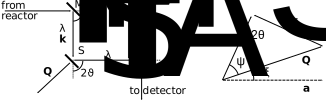
\includegraphics[width = 0.75 \textwidth]{figures/tas_triangle}
	\end{center}
	\caption[TAS layout and scattering triangle.]{
		Triple-axis layout (left) and corresponding scattering triangle (right).
		Figures inspired by Ref. \cite[p. 72, Fig. 3.8]{Shirane2002} and \cite[p. 15, Fig. 1.6]{Shirane2002}, respectively.
		\label{fig:scattering_triangle}}
\end{figure}

We can calculate $2 \theta_S$ via the cosine theorem \cite[pp. 694-695]{Arens2015}, i.e.
by forming the scalar product of $\left| Q \right>$ with itself in lab units \cite[p. 11]{Shirane2002}:
\begin{equation} 
	\left| Q \right> \ =\  \left| k_i \right> - \left| k_f \right>,
\end{equation}
\begin{equation} 
	\left< Q | Q \right> \ =\  \left( \left< k_i \right| - \left< k_f \right| \right) \cdot \left( \left| k_i \right> - \left| k_f \right> \right)
	\ =\  \left< k_i | k_i \right> + \left< k_f | k_f \right> - 2 \left< k_i | k_f \right>,
\end{equation}
\begin{equation} 
	Q^2 \ =\  k_i^2 + k_f^2 - 2 k_i k_f \cos \left( 2 \theta_S \right),
\end{equation}
\begin{equation}
	\boxed{ 2 \theta_S \ =\  \sigma_s \cdot \arccos \left( \frac{k_i^2 + k_f^2 - Q^2}{2 k_i k_f} \right). }
\end{equation}

We could now -- as is done in the work by Lumsden \textit{et al.} \cite{Lumsden2005} -- calculate the length
$Q$ of the vector $\left| Q \right>$ by explicitly transforming it into lab units using Eq. \ref{eq:UBtrafo}.
Instead, we directly determine its length in lab units from its native rlu system using the covariant dot 
product \cite[p. 808]{Arens2015}:
\begin{equation}
	Q %\ =\ Q_{\mathrm{lab}} 
	\ =\ 
	\sqrt{Q^{\mathrm{rlu}}_i Q_{\mathrm{rlu}}^i} \ =\  \sqrt{g_{ij} Q_{\mathrm{rlu}}^i Q_{\mathrm{rlu}}^j}.
\end{equation}

As we could scatter in either clockwise or counter-clockwise direction, $2 \theta_S$ can be positive or negative.
The sign of $2 \theta_S$ is given by the sample scattering sense $\sigma_s = \pm 1$.


%\vspace{0.5cm}


The final and most complicated angle to determine is the sample rotation $\Theta_S$.
It is given by the angle of the incoming wavevector $\left| k_i \right>$ to an (arbitrary) direction 
$\left| a \right>$ which is known from sample orientation, this is usually a Bragg peak \cite[p. 87]{Shirane2002}.
If we were to explicitly use the $U$ matrix here, this vector would be one of its rows.
The situation is shown in the right panel of Fig. \ref{fig:scattering_triangle}.
We split $\Theta_S$ into the angle $\psi$ between $\left| k_i \right>$ and $\left| Q \right>$ 
and the angle $\xi$ between $\left| Q \right>$ and $\left| a \right>$:
\begin{equation} \boxed{ \Theta_S \ =\  180^{\circ} - \left( \psi + \xi \right).} \end{equation}


%\vspace{0.5cm}


The angle $\psi$ between $\left| k_i \right>$ and $\left| Q \right>$ is determined from the scattering triangle, as before
in lab units:
\begin{equation}
	\left| k_f \right> \ =\  \left| k_i \right> - \left| Q \right>,
\end{equation}
\begin{equation} 
	\left< k_f | k_f \right> \ =\  \left( \left< k_i \right| - \left< Q \right| \right) \cdot \left( \left| k_i \right> - \left| Q \right> \right)
	\ =\  \left< k_i | k_i \right> + \left< Q | Q \right> - 2 \left< k_i | Q \right>,
\end{equation}
\begin{equation}
	k_f^2 \ =\  k_i^2 + Q^2 - 2 k_i Q \cos \psi,
\end{equation}
\begin{equation}
	\boxed{ \psi \ =\  \sigma_s \cdot \arccos \left( \frac{k_i^2 + Q^2 - k_f^2}{2 k_i Q} \right).}
\end{equation}


%\vspace{0.5cm}


The angle $\xi$ between $\left| Q \right>$ and orientation vector $\left| a \right>$ is also determined 
from the properties of the scalar product.
Here we have to use its covariant form via the metric tensor, $g_{ij}$, \cite[p. 808]{Arens2015},
because $\left| a \right>$ is a coordinate in crystal space naming a Bragg reflection,
while $\left| Q \right>$ would natively live, as before, in instrument space, where we can thus avoid transforming to,
unlike Ref. \cite{Lumsden2005}.
\begin{equation} 
	\boxed{ \xi \ =\  
\sigma_{\mathrm{side}} \cdot \arccos \left( \frac{ \left< Q_{\mathrm{rlu}} | a \right> }{ \sqrt{\left< Q_{\mathrm{rlu}} | Q_{\mathrm{rlu}} \right>} \sqrt{\left< a | a \right>} } \right) \ =\  
\sigma_{\mathrm{side}} \cdot \arccos \left( \frac{ Q_{\mathrm{rlu}}^i g_{ij} a^j }{ \sqrt{Q_{\mathrm{rlu}}^i g_{ij} Q_{\mathrm{rlu}}^j} \sqrt{a^i g_{ij} a^j} } \right).}
\label{eq:xi}
\end{equation}

The sign, $\sigma_{\mathrm{side}}$, of $\xi$ depends on which side of the orientation vector 
$\left| a \right>$ the scattering vector $\left| Q_{\mathrm{rlu}} \right>$ is located. 
The sign can be found by calculating the (covariant) cross product of $\left| a \right>$ and 
$\left| Q_{\mathrm{rlu}} \right>$ to give an out-of-plane vector $\left| x \right>$ which can be compared with 
the given scattering plane up vector.
The covariant cross-product is calculated as \cite[p. 815]{Arens2015}:
\begin{equation}
	x^l \ =\  g^{li} \epsilon_{ijk} a^j Q_{\mathrm{rlu}}^k,
\end{equation}
where $\epsilon_{ijk}$ is the general Levi-Civita symbol formed from the determinant of the 
basis vectors $\left| \underline{b}_i \right>$, see Ref. \cite[p. 815]{Arens2015}:
\begin{equation}
	\epsilon_{ijk} \ =\  \left|
		\begin{array}{ccc} \left| 
			\underline{b}_i \right> & \left| \underline{b}_j \right> & \left| \underline{b}_k \right>
		\end{array} \right|.
\end{equation}



\paragraph*{Special case}
For cubic crystals with $\alpha = \beta = \gamma = 90^{\circ}$ and the lattice constants all equal, 
$a = b = c$, the metric tensor is diagonal, $g_{ij} = \delta_{ij} \cdot \left( 2\pi / a \right)^2$.
With that Eq. \ref{eq:xi} simplifies to:
\begin{equation}
	\xi \ =\  \sigma_{\mathrm{side}} \cdot \arccos \left( \frac{ Q^{\mathrm{rlu}}_i a^i }{ \sqrt{Q^{\mathrm{rlu}}_i Q_{\mathrm{rlu}}^i} \sqrt{a_i a^i} } \right).
\end{equation}
% ------------------------------------------------------------------------------------------------------------------------------------


\section{Summary}
This chapter introduced some important concepts from solid-state physics and crystallography that are essential
for an understanding of the basic coordinate system transformations from the generally non-orthogonal (real or 
reciprocal) crystal coordinates to the orthonormal lab coordinates used at the instrument.
In practice, it is the crystal coordinates that are entered into the instrument control software by
the user, not the raw instrument angles. A pathfinding system for triple-axis spectrometers thus has to know both.
Internally, it will be more convenient for the software to use instrument-related coordinates, as we will see in 
the following chapters, but the input and output will be in crystal coordinates.

Having established all the necessary physical foundations, the next chapter will proceed to do the same for the 
essential concepts in computer science before putting everything together in a pathfinding algorithm.


\chapter{Path-finding}
%
% path-finding
% @author Tobias Weber <tweber@ill.fr>
% @date 2021
% @license see 'LICENSE' file
%
\chapter{Path-finding and Algorithm Overview}

This chapter is devoted to the development of the theoretical frameworks for path-finding in a triple-axis spectrometer (TAS). 
The path should furthermore be optimal in the sense that the instrument not only avoids obstacles like walls or equipment in 
the experimental area, but also keeps a maximum distance from them.

Before looking at the situation with TAS in section \ref{sec:tasrobot}, we shortly review the ideas of motion planning for a 
point-like robot in section \ref{sec:pointrobot}.



\section{Motion planning for a point-like robot}
\label{sec:pointrobot}

\subsection*{Sector-based method}
An algorithm for motion planning in a point-like robot based on decomposing the available space into sectors is 
given in Ref. \cite[Ch. 13, pp. 283-306]{Berg2008}, whose descriptions we follow in this section. 
While the book chapter also describes polygonal robots, we limit ourselves to the parts of the chapter 
that are relevant for the present work.

The movement of the point-like robot in question is not restricted to conventional Cartesian space, its coordinates are given in configuration
space  \cite[Ch. 13.1, pp. 284-286]{Berg2008}, which comprises its inherent degrees of freedom and can -- for instance -- include angular motion.

The algorithm consists of two parts: First, the separation of allowed space into sectors, within which the robot can move 
without hitting an obstacle \cite[p. 286]{Berg2008}. 
The second part concerns the computation of the actual path and is given in Ref. \cite[p. 289]{Berg2008}. 
In the first part, a trapezoidal map (explained below) is created for the configuration space containing the obstacles, 
both of polygonal shape. The trapezoids inside the obstacles are removed form the final map as the robot has to stay clear 
of them. The second part of the algorithm calculates the path of the robot by finding the trapezoids which contain the start 
and goal points, and finding the edges between adjacent trapezoids from starting to ending trapezoid via a breadth-first search in the 
trapezoidal map. The robot will thus first move to the centre of its containing trapezoid, followed by the centre of an edge connecting 
the current to the next trapezoid, next to the centre of the next trapezoid, and so forth until it arrives at its goal. 
The situation is depicted in Fig. \ref{fig:robot_trapezoids}, where we restrict ourselves to line-like obstacles for simplicity, effectively
only using the second part of the algorithm.

Trapezoidal maps and the algorithm for their calculation are given in Ref. \cite[Ch. 6, pp. 121-146]{Berg2008}. Basically, the map of
trapezoids is obtained by extending vertical lines from every vertex in a collection of line segments. The vertical
extensions reach out until they intersect with another line segment of the collection, or an outer bounding box. The original line 
segment and the intersected segment on top (or bottom, respectively) together with the vertical lines form a trapezoid, as shown in 
Fig. \ref{fig:robot_trapezoids}. Together with the trapezoid map, the algorithm constructs in $O \left(n \log_{2} n \right)$ time a data 
structure, which allows querying for the trapezoid containing a given point with time complexity $O \left( \log_{2} n \right)$, 
where $n$ is the number of line segments \cite[Theorem 6.3, p. 133]{Berg2008}.

\begin{figure*}[htb]
	\centering
	\includegraphics[width = 0.4 \textwidth]{figures/pointrobot_walls.pdf}
	\hspace{1 cm}
	\includegraphics[width = 0.4 \textwidth]{figures/pointrobot_walls_trapezoids.pdf}
	\caption{Left panel: A point-like robot has to find a way around line segments which represent obstacles. Right panel: 
		The algorithm outlined in Ref. \cite[p. 289]{Berg2008} constructs a trapezoid map and moves the robot on the
		shortest path from the centre of one trapezoid to the centre of the edge connecting to the next trapezoid, to the
		centre of that trapezoid, and so forth (blue arrows).}
	\label{fig:robot_trapezoids}
\end{figure*}

While the present algorithm can be extended towards polygonal robots \cite[Ch. 13.3, pp. 290-297]{Berg2008} and provides
some useful ideas, it has several severe drawbacks. First and foremost, the trapezoid map cannot handle the case when
two or more line segment vertices coincide, making it very difficult to model polygonal obstacles and not only using mere
line segments. Second, our own implementation has shown that for the algorithm to be stable, it has to handle many 
special cases, for example to eliminate vertices with equal $x$ coordinate components or vertical lines.

\vspace{0.5cm}

\subsection*{Retraction method}
Apart from decomposing the available configuration space into sectors, a more direct approach can be taken. This
approach is called the retraction method and is based on constructing the Voronoi regions (see \ref{ch:voronoi})
of the obstacles and moving the robot along the Voronoi edges, which ensures that the path is optimal in the
sense that the robot is always at the farthest distance from any obstacle \cite[pp. 163 and 304]{Berg2008}.
An example path for the same problem as before is given in Fig. \ref{fig:robot_voronoi}.
It is this approach we will follow for TAS motion planning.

\begin{figure}[htb]
	\centering
	\includegraphics[width = 0.4 \textwidth]{figures/pointrobot_walls_voronoi.pdf}
	\caption{The accessible configuration space is subdivided into the Voronoi regions of the obstacles (coloured). The optimal
		path (blue arrows) in the sense that it keeps the robot at maximum distance from any obstacle, has it move along the 
		Voronoi edges.}
	\label{fig:robot_voronoi}
\end{figure}



\section{Motion planning for a triple-axis spectrometer}
\label{sec:tasrobot}

As it is imperative that the instrument not move into any walls, we choose the retraction method using the obstacles' Voronoi regions.
As for a TAS several coordinate systems are available, we have several equivalent possibilities to describe its movement. 

\subsection*{Instrument positions configuration space}
The first possibility would be to model the entire instrument as a polygonal robot arm and directly use the position of the robot as
its configuration space. This way it would be directly possible to use a polygonal representation of the walls and construct their
Voronoi regions -- or even trapezoidal maps -- as discussed in Sec. \ref{sec:pointrobot}. The main problem with this approach is the
very complicated treatment necessary for the instrument itself.

\subsection*{Crystal coordinates configuration space}
A better way is to use a configuration space where the instrument is represented as a single point in that space. This comes at the 
cost of the shape of the walls becoming more complicated when transformed into configuration space, 
they may not even be simply-connected anymore in that space. There
are two choices for such a configuration space: We can either use the reciprocal crystal coordinates as discussed in Ch. \ref{ch:xtal}
or use a configuration space comprised of the instrumental angles.

Using the reciprocal crystal coordinates as configuration space would need a transformation of the walls into the four-dimensional
reciprocal space (three momentum and on energy coordinate). Even when taking into account that the TAS is usually restricted
to a two-dimensional scattering plane, thereby dropping one of the momentum dimensions, the problem would still be 
three-dimensional.

\subsection*{Angular configuration space}
On the other hand, using the instrument angles seems to be even more complicated at first glance. The instrument comprises
six angles, namely the crystal and scattering angles for the monochromator, the sample and the analyser crystals, respectively,
leading to a six-dimensional configuration space. When can take into account that not all angles are independent of one another:
The monochromator and analyser scattering angles are always double their respective crystal angles, because they both
have to fulfill the Bragg condition. We are therefore left with four independent angles: the monochromator and analyser 
scattering angles as well as the sample crystal and scattering angle. 

We are mainly interested in collisions of the instrument with walls or itself, this way the sample crystal angle can be dropped 
from the analysis, because it only rotates the sample axis, but does not move the instrument. It can still lead to forbidden 
positions if it rotates too far and rips out cables or tubes, but these cases we can treat as their own one-dimensional problem. 

A further simplification is possible when taking into account that during a typical experiment the instrument usually only moves 
either its monochromator or analyser angle to choose the energy transfer, but not both. Therefore, one of these angles, 
usually the analyser angle, rests at a constant value. In total, we are left with a two-dimensional configuration space comprised 
of the monochromator and the sample scattering angle. A typical situation is shown in Fig. \ref{fig:tas_wall}. Here, the instrument 
motion is blocked by an obstacle in the experimental zone. The configuration space image shows that the obstacle transforms
into a non-primitive geometric object in configuration space, which -- as already mentioned -- does not even have to be
simply-connected.

\begin{figure}[htb]
	\centering
	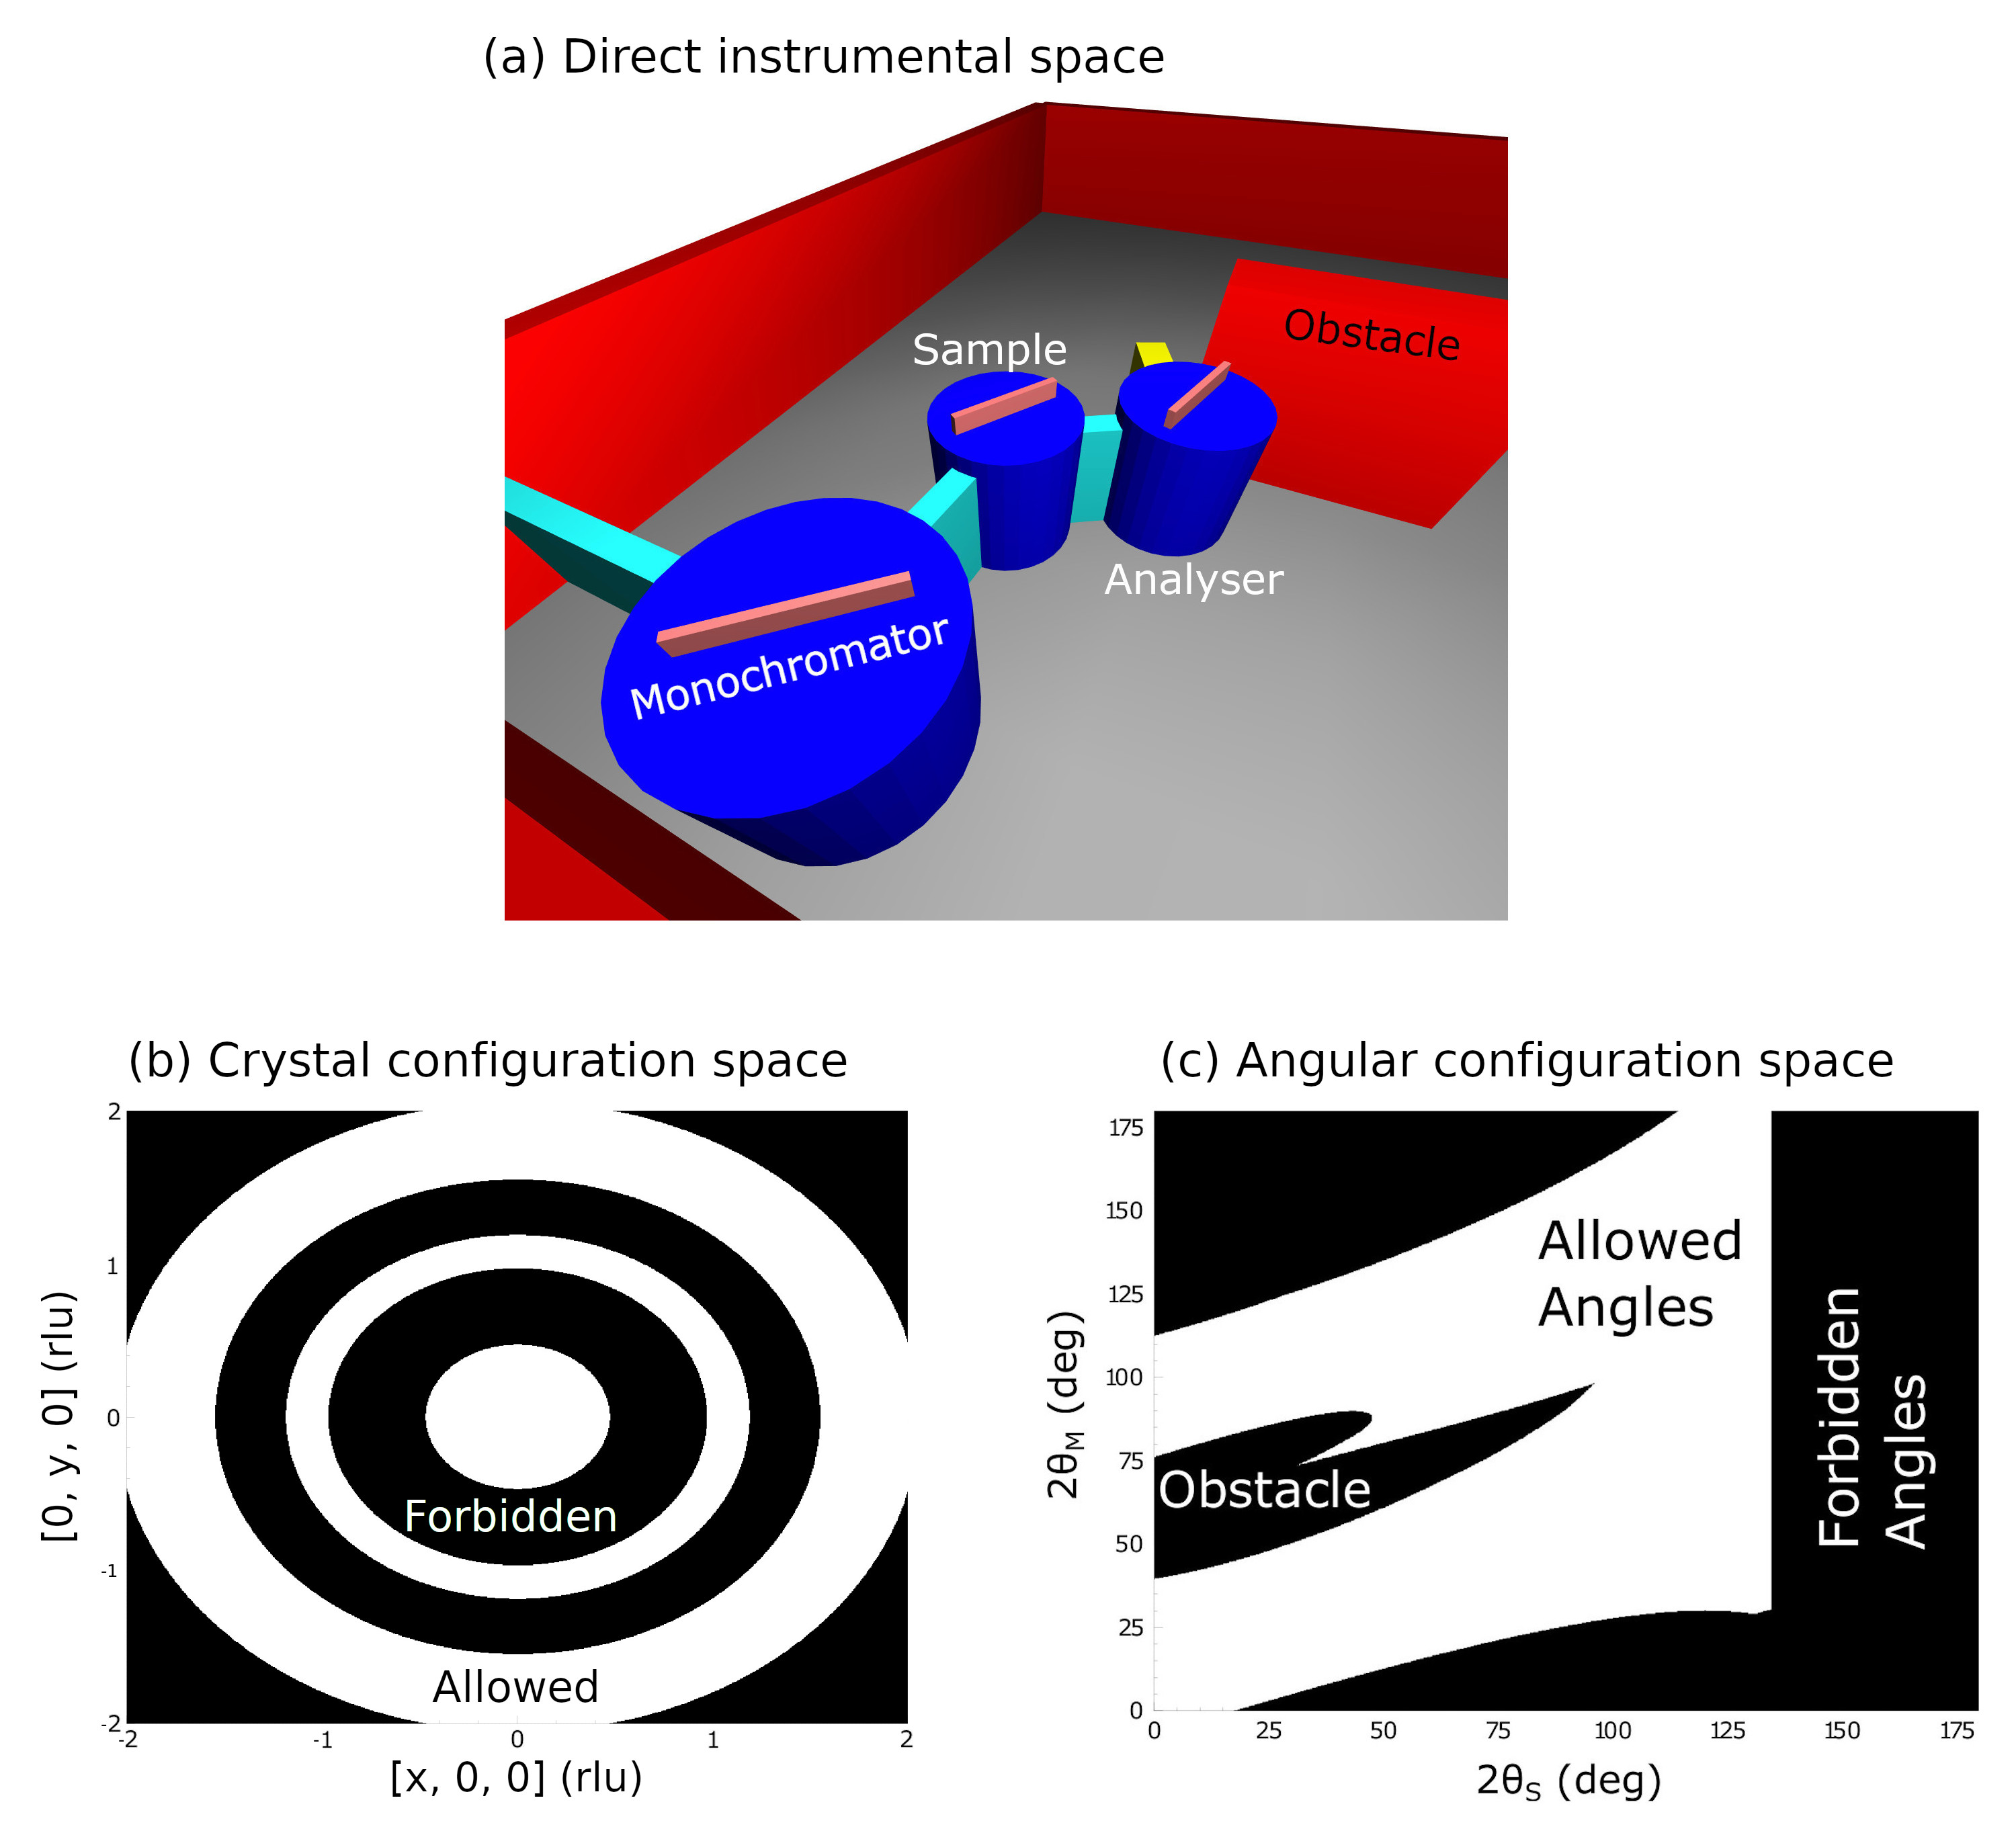
\includegraphics[width = 0.95 \textwidth]{figures/tas_wall.jpg}
	\caption{An obstacle as it appears in the instrument space (left) and in the angular configuration space (right). 
		In the configuration space, allowed instrument angular positions are shown in white, forbidden positions in black. 
		The outer areas of disallowed positions are given either by collisions of the instrument with the outer walls or 
		with itself.}
	\label{fig:tas_wall}
\end{figure}


\subsection*{Overall strategy}

The strategy for planning the motion of the spectrometer comprises several steps. Modifying the algorithm for
a point-like robot described in Ref. \cite[Ch. 13, pp. 283-306]{Berg2008} (see Sec. \ref{sec:pointrobot}), we summarise the
steps here before describing them in detail together with the actual implementation in the next chapter.

Two tasks are needed. The first task is building the possible paths the instrument can move along. The second task contains the movement of the instrument on the generated paths. The two tasks comprise these following steps:
\begin{enumerate}
	\item Building the path.
	\begin{enumerate}
		\item Calculate the angular configuration space as described above.
		\item Trace the obstacle contours in angular configuration space. This step is necessary because they can be of arbitrary
			shape in this representation and are not necessarily geometric primitives, as seen in Fig. \ref{fig:tas_wall}.
		\item Approximate the traced contour curves with line segments.
		\item Simplify the line segments. This is necessary because the line segments generated in the previous step are not optimal:
			First, they may contain back-to-back collinear lines which can be unified. Second, jagged edges and zigzag lines may be
			produced in practice. These need to be eliminated or at least smoothed before the next step.
		\item Split all polygonal line segments that build up the contours into convex regions. With this we can group all lines
			in a convex region and only calculate the Voronoi diagrams for these groups instead of all line segments.
		\item Calculate the Voronoi diagram (see Ch. \ref{ch:voronoi}) for the line segment groups. The Voronoi edges are the
		possible instrument paths in configuration space. Save both the Voronoi diagram as well as its representation in a graph structure.
		\item Simplify the Voronoi diagram. For example, Voronoi vertices and edges inside obstacle regions have to be removed.
			These are generated in the previous step because, there, no differentiation was made between the ``inside'' and
			``outside'' regions of the convex line segment contour groups.
	\end{enumerate}

	\item Executing the instrument motion.
	\begin{enumerate}
		\item Convert the given crystal coordinates into instrument coordinates.
			The user of a triple-axis spectrometer usually enters the coordinates in the crystal coordinate system
			(see Ch. \ref{ch:xtal}). The start and end point of the instrument path have to be converted from crystal
			coordinates into instrument angles. The instrument angles form a coordinate point in angular configuration
			space.
		\item Determine the Voronoi regions of the start and end coordinate points.
		\item Move the instrument to the edge of the start Voronoi region.
		\item Calculate the shortest path to the edge of the Voronoi region containing the end point using Dijkstra's algorithm
			(see Ch. \ref{ch:dijkstra}) and move the instrument along that path.
		\item Move the instrument from the edge of the Voronoi region containing the end point towards that point.
	\end{enumerate}
\end{enumerate}


\chapter{Implementation}
% library
% GUI
% Nomad interface
% Verweis auf Nomad 3D und vTAS/vEXP


\appendix
%\part{Back matter}
%\addcontentsline{toc}{part}{Back matter} 
%
% notation
% @author Tobias Weber <tweber@ill.fr>
% @date mar-2021
% @license see 'LICENSE' file
%

\chapter{Notation}

\begin{tabular}{|c|c|}
\hline
\bf{Notation} & \bf{Explanation} \tabularnewline
\hline
$ \underline{v} $ & A vector. \tabularnewline
\hline
$ M = \left( m_{ij} \right) $ & A matrix. \tabularnewline
\hline
$\left| x \right> \,=\, \left( x^i \right) $ & A contravariant vector. \tabularnewline
\hline
$\left< x \right| \,=\, \left( x_i \right) $ & A covariant vector. \tabularnewline
\hline
$s \,=\, \left< x | y \right> \,=\, x_i y^i \,=\, g_{ij} x^i y^j $ & A scalar/inner product, the sums over $i$ and $j$ are implied \cite{wiki_summation}. \tabularnewline
\hline
$\left(a^{i}_{\;j}\right) \,=\, \left| x \right> \left< y \right| \,=\, x^i y_j$ & A tensor/outer product. \tabularnewline
\hline
\end{tabular}

\chapter{List of publications}
The latest list of publications can be found on-line under \url{https://orcid.org/0000-0002-7230-1932}. 
We reproduce the current version as of July 2021 in the following.


\section{Works as principal author}
\subsection*{Papers}
\begin{itemize}
	\item T. Weber, \textit{Update 2.0 to ``Takin: An open-source software for experiment planning, visualisation, and data analysis'', (PII: S2352711016300152)},
	SoftwareX, Volume 14, 100667 (June 2021),
	DOI: \href{https://doi.org/10.1016/j.softx.2021.100667}{10.1016/j.softx.2021.100667}.

	\item T. Weber, J. Waizner, P. Steffens, A. Bauer, C. Pfleiderer, M. Garst, and P. B\"oni, 
	\textit{Polarized inelastic neutron scattering of nonreciprocal spin waves in MnSi},
	Physical Review B, Volume 100, 060404(R) (12 August 2019),
	DOI: \href{https://doi.org/10.1103/PhysRevB.100.060404}{10.1103/PhysRevB.100.060404}.

	\item  T. Weber, J. Waizner, G. S. Tucker, L. Beddrich, M. Skoulatos, R. Georgii, A. Bauer, C. Pfleiderer, M. Garst, and P. B\"oni, 
	\textit{Non-reciprocal magnons in non-centrosymmetric MnSi},
	AIP Advances, Volume 8, 101328 (9 October 2018),
	DOI: \href{https://doi.org/10.1063/1.5041036}{10.1063/1.5041036}.

	\item T. Weber, J. Waizner, G. S. Tucker, R. Georgii, M. Kugler, A. Bauer, C. Pfleiderer, M. Garst, and P. B\"oni, 
	\textit{Field dependence of nonreciprocal magnons in chiral MnSi},
	Physical Review B, Volume 97, 224403 (5 June 2018),
	DOI: \href{https://doi.org/10.1103/PhysRevB.97.224403}{10.1103/PhysRevB.97.224403}.

	\item T. Weber, B. Roessli, C. Stock, T. Keller, K. Schmalzl, F. Bourdarot, R. Georgii, R. A. Ewings, R. S. Perry, and P. B\"oni, 
	\textit{Transverse acoustic phonon anomalies at intermediate wave vectors in $MgV_2O_4$},
	Physical Review B, Volume 96, 184301 (7 November 2017),
	DOI: \href{https://doi.org/10.1103/PhysRevB.96.184301}{10.1103/PhysRevB.96.184301}.
	
	\item T. Weber, \textit{Update 1.5 to ``Takin: An open-source software for experiment planning, visualisation, and data analysis'', (PII: S2352711016300152)},
	SoftwareX, Volume 6, Pages 148-149 (10 July 2017),
	DOI: \href{https://doi.org/10.1016/j.softx.2017.06.002}{10.1016/j.softx.2017.06.002}.

	\item T. Weber, R. Georgii, and P. B\"oni,
	\textit{Takin: An open-source software for experiment planning, visualisation, and data analysis},
	SoftwareX, Volume 5, Pages 121-126 (14 July 2016),
	DOI: \href{https://doi.org/10.1016/j.softx.2016.06.002}{10.1016/j.softx.2016.06.002}.

	\item T. Weber, G. Brandl, R. Georgii, and P. B\"oni,
	\textit{An open-source software package for data treatment in a MIEZE experiment},
	Journal of Physics: Conference Series, Volume 528, 012034 (2014),
	DOI: \href{https://doi.org/10.1088/1742-6596/528/1/012034}{10.1088/1742-6596/528/1/012034}.
	
	\item T. Weber, G. Brandl, R. Georgii, W. H\"au\ss{}ler, S. Weichselbaumer, P. B\"oni,
	\textit{Monte-Carlo simulations for the optimisation of a TOF-MIEZE instrument},
	Nuclear Instruments and Methods in Physics Research Section A: Accelerators, Spectrometers, Detectors and Associated Equipment Volume Volume 713, Pages 71-75 (11 June 2013),
	DOI: \href{https://doi.org/10.1016/j.nima.2013.03.010}{10.1016/j.nima.2013.03.010}.
\end{itemize}


\subsection*{Theses}
\begin{itemize}
	\item T. Weber, \textit{Dynamics at the Orbital Ordering Phase Transition in $MgV_2O_4$ and at the Ferromagnetic Phase Transition in $MnSi$} (20 March 2017), ISBN: 978-3-8439-3114-4,
	PhD Thesis in Physics, Technische Universit\"at M\"unchen, Physikdepartment E21,
	Garching, Germany. URL: \url{http://nbn-resolving.de/urn/resolver.pl?urn:nbn:de:bvb:91-diss-20170320-1339645-0-4}.

	\item T. Weber, \textit{MIEZE in Theory, Simulation and Experiment} (5 December 2012), 
	Diploma Thesis in Physics, Technische Universit\"at M\"unchen, Physikdepartment E21,
	Garching, Germany.
\end{itemize}



\section{Works as contributing author}

\begin{itemize}
	\item Y. Nambu, J. Barker, Y. Okino, T. Kikkawa, Y. Shiomi, M. Enderle, T. Weber, B. Winn, M. Graves-Brook, J. M. Tranquada, T. Ziman, M. Fujita, G. E. W. Bauer, E. Saitoh, and K. Kakurai, 
	\textit{Observation of Magnon Polarization},
	Physical Review Letters, Volume 125, 027201 (6 July 2020),
	DOI: \href{https://doi.org/10.1103/PhysRevLett.125.027201}{10.1103/PhysRevLett.125.027201}.

	\item G. Song, L. Porcar, M. B\"ohm, F. Cecillon, C. Dewhurst, Y. Le Goc, J. Locatelli, P. Mutti, and T. Weber, 
	\textit{Deep Learning Methods On Neutron Scattering Data},
	EPJ Web of Conferences, Volume 225, 01004 (20 January 2020),
	DOI: \href{https://doi.org/10.1051/epjconf/202022501004}{10.1051/epjconf/202022501004}.

	\item D. W. Tam, H.-H. Lai, J. Hu, X. Lu, H. C. Walker, D. L. Abernathy, J. L. Niedziela, T. Weber, M. Enderle, Y. Su, Z. Q. Mao, Q. Si, and P. Dai,
	\textit{Plaquette instability competing with bicollinear ground state in detwinned FeTe},
	Physical Review B, Volume 100, 054405 (5 August 2019),
	DOI: \href{https://doi.org/10.1103/PhysRevB.100.054405}{10.1103/PhysRevB.100.054405}.
	
	\item R. Georgii and T. Weber,
	\textit{The Helical Magnet MnSi: Skyrmions and Magnons},
	Quantum Beam Science 2019, 3(1) (21 February 2019),
	DOI: \href{https://doi.org/10.3390/qubs3010004}{10.3390/qubs3010004}.
	
	\item R. Georgii, T. Weber, G. Brandl, M. Skoulatos, M. Janoschek, S. Mühlbauer, C. Pfleiderer, and P. B\"oni,
	\textit{The multi-purpose three-axis spectrometer (TAS) MIRA at FRM II},
	Nuclear Instruments and Methods in Physics Research Section A: Accelerators, Spectrometers, Detectors and Associated Equipment Volume 881, Pages 60-64 (11 February 2018),
	DOI: \href{https://doi.org/10.1016/j.nima.2017.09.063}{10.1016/j.nima.2017.09.063}.
\end{itemize}

\chapter{Errata and Online Resources}
Up-to-date errata for this work, comprising the thesis text and the software, 
will be published on-line under the DOI \href{https://doi.org/10.5281/zenodo.4625649}{10.5281/zenodo.4625649}.
Additionally, the main software repository is available here: \url{https://code.ill.fr/scientific-software/takin/paths},
a mirror of the repository can also be found here: \url{https://github.com/tweber-ill/ill_mirror-takin2-paths}.


%\section{Bibliography}
\bibliographystyle{ieeetr}
\bibliography{\jobname.bib}
% ====================================================================================================================================

\end{document}
